%! suppress = LineBreak
\section{Разработка игры}

WebGL сборку проекта можно посмотреть здесь\cite{s9}.

\subsection{Документация}
Для публикации Unity требует документацию ассета на английском. Для написания документации использовалась система генерации статических сайтов Jekyll\cite{s11} и тема Just the Docs\cite{s12}. Документация доступна здесь\cite{s13}.


\subsection{Демонстрационные сцены}
Для демонстрационных целей было создано три сцены:

\begin{enumerate}[label=\textbullet]
    \item \textbf{Weapon Demo} -- сцена, в которой демонстрируется 140 оружий, заранее созданных разработчиком. Кроме того, в этой сцене есть визуализация силовых полей, действующих на снаряды.

    \begin{figure}[ht]
        \begin{center}
            \scalebox{0.15}{
                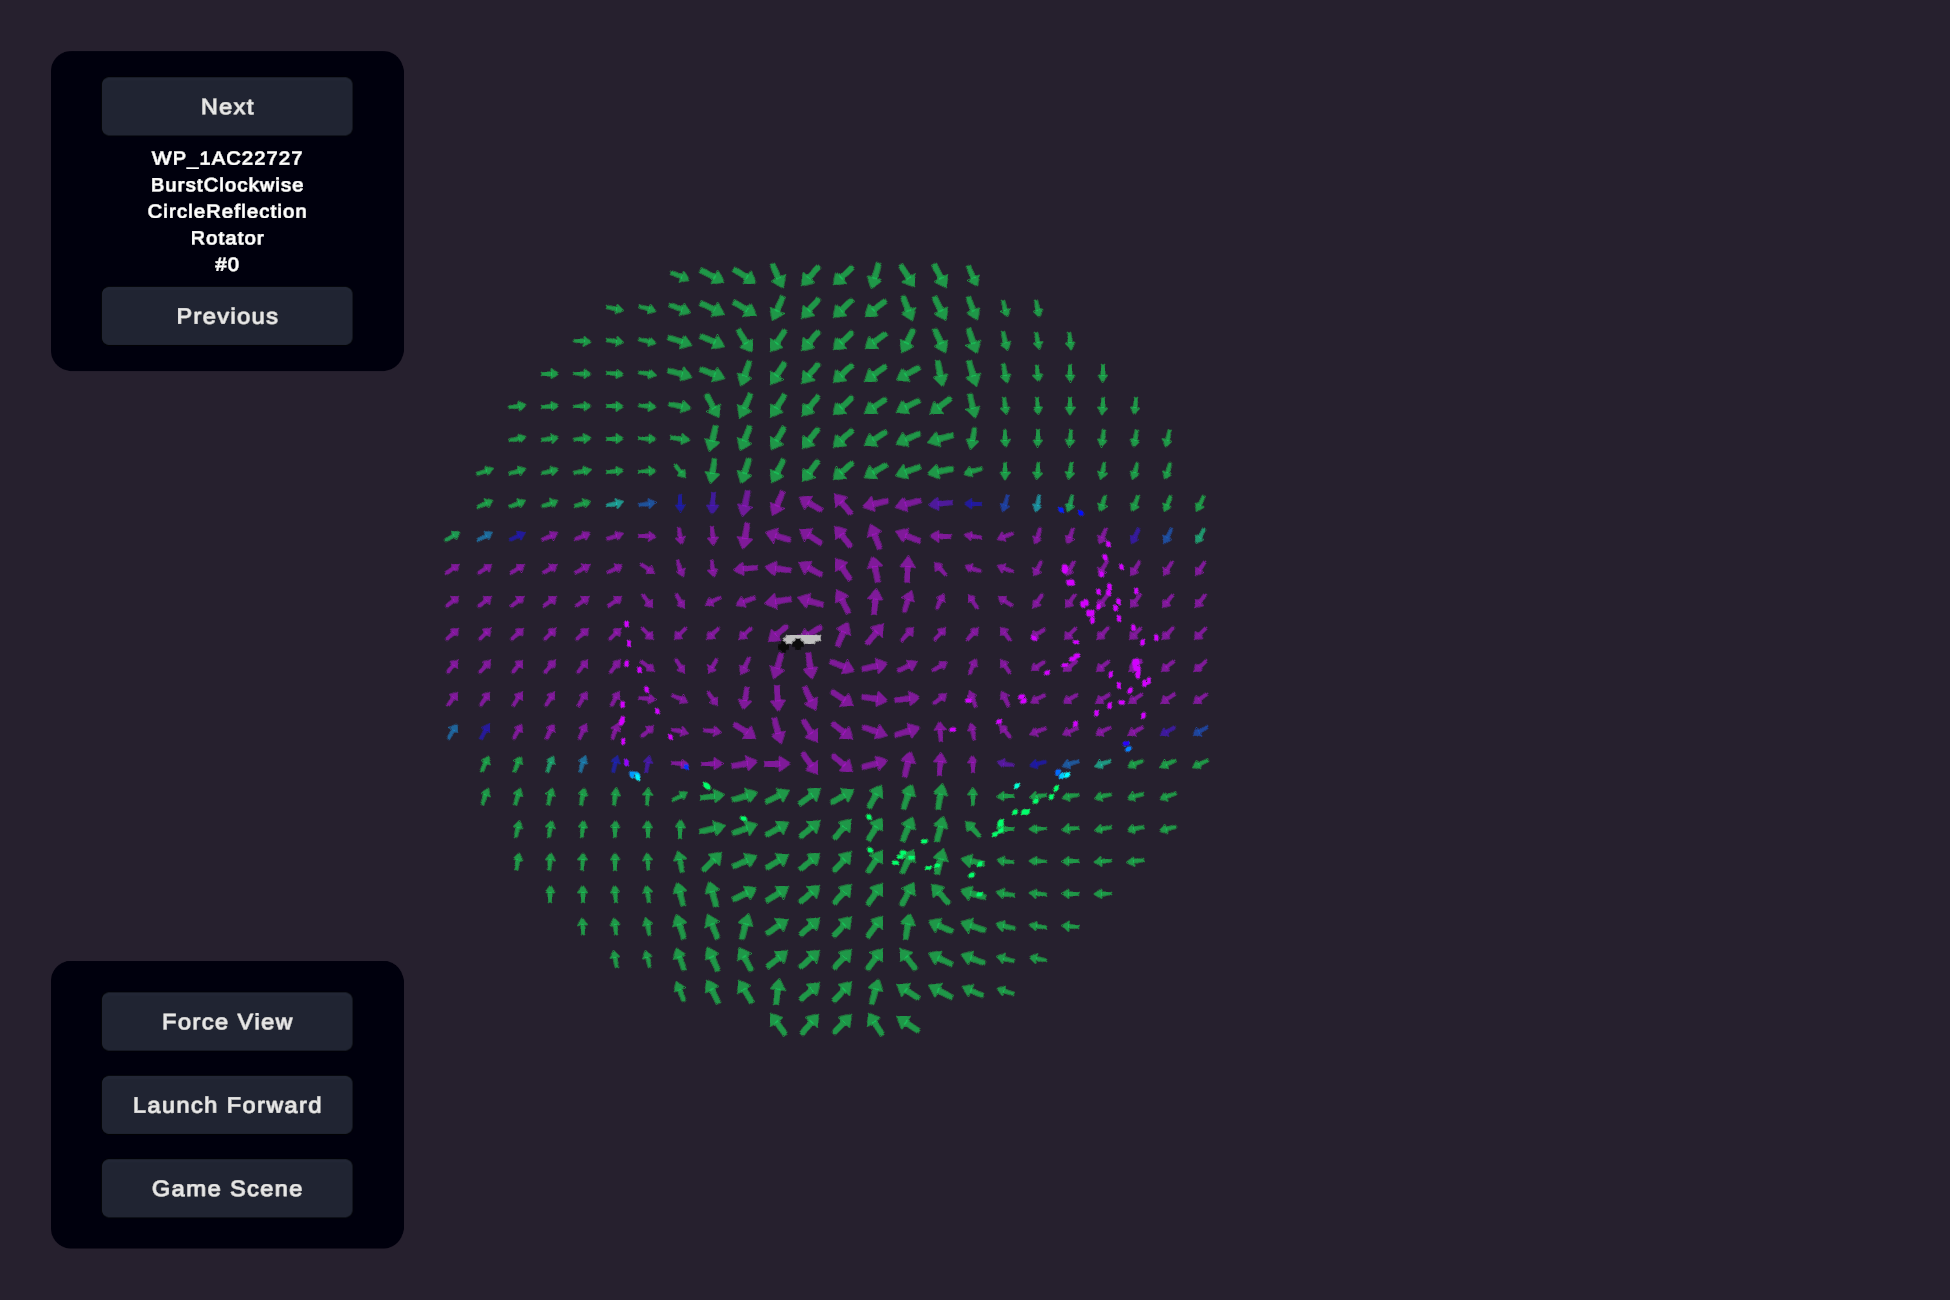
\includegraphics{images/WeaponDemo}
            }

            \caption{
                \label{WeaponDemo}
                Weapon Demo.}
        \end {center}
    \end {figure}

    \textbf{Замечание.} Разные группы снарядов могут иметь разные значения параметров {\small \textbf{SignY}} и {\small \textbf{SignX,}} поэтому визуализация силового поля может быть некорректна для каких-то из них.


    \item \textbf{Shadow Survival} -- простая игра в жанре <<Shoot ’em up>>. Во время игры генерируется оружие, которое можно подобрать и настроить некоторые параметры.

    \begin{figure}[ht]
        \begin{center}
            \scalebox{0.2}{
                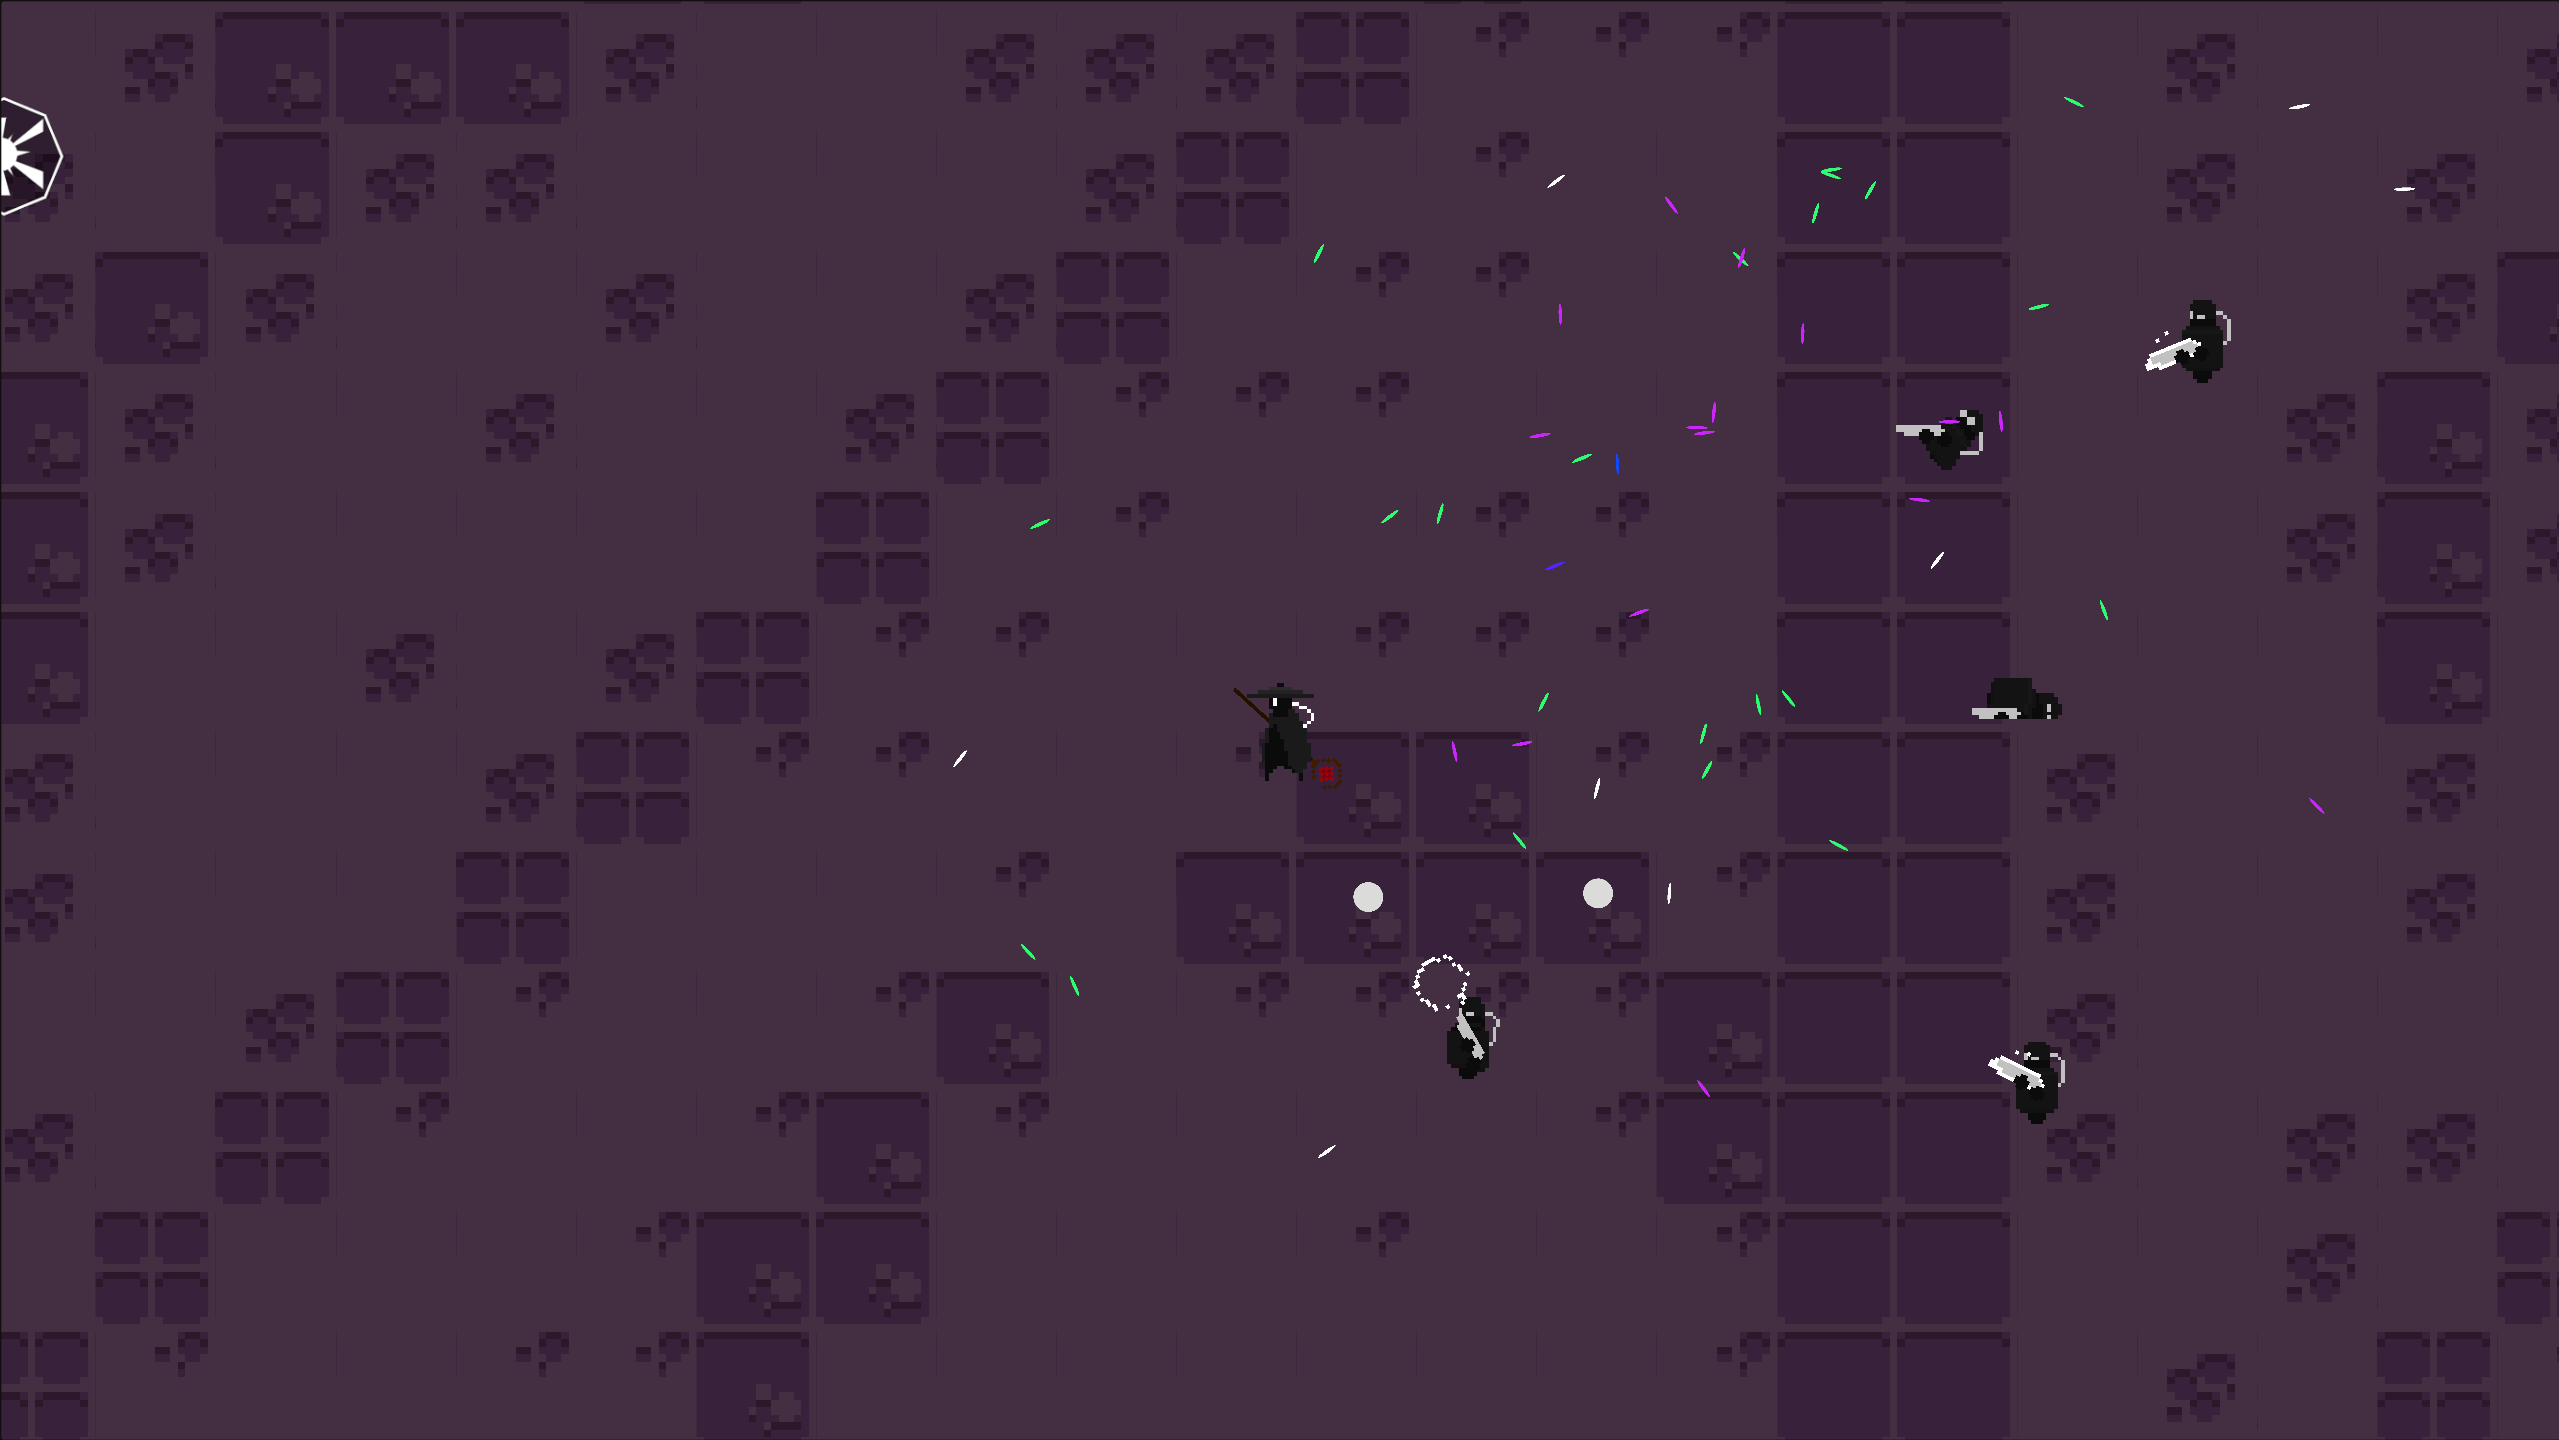
\includegraphics{images/ShadowSurvival}
            }

            \caption{
                \label{ShadowSurvival}
                Shadow Survival.
            }
        \end {center}
    \end {figure}

    \item \textbf{Space Shooter} -- простая игра тоже в жанре <<Shoot ’em up>>. Здесь оружие генерируется у врагов случайным образом.

    \begin{figure}[ht]
        \begin{center}
            \scalebox{0.2}{
                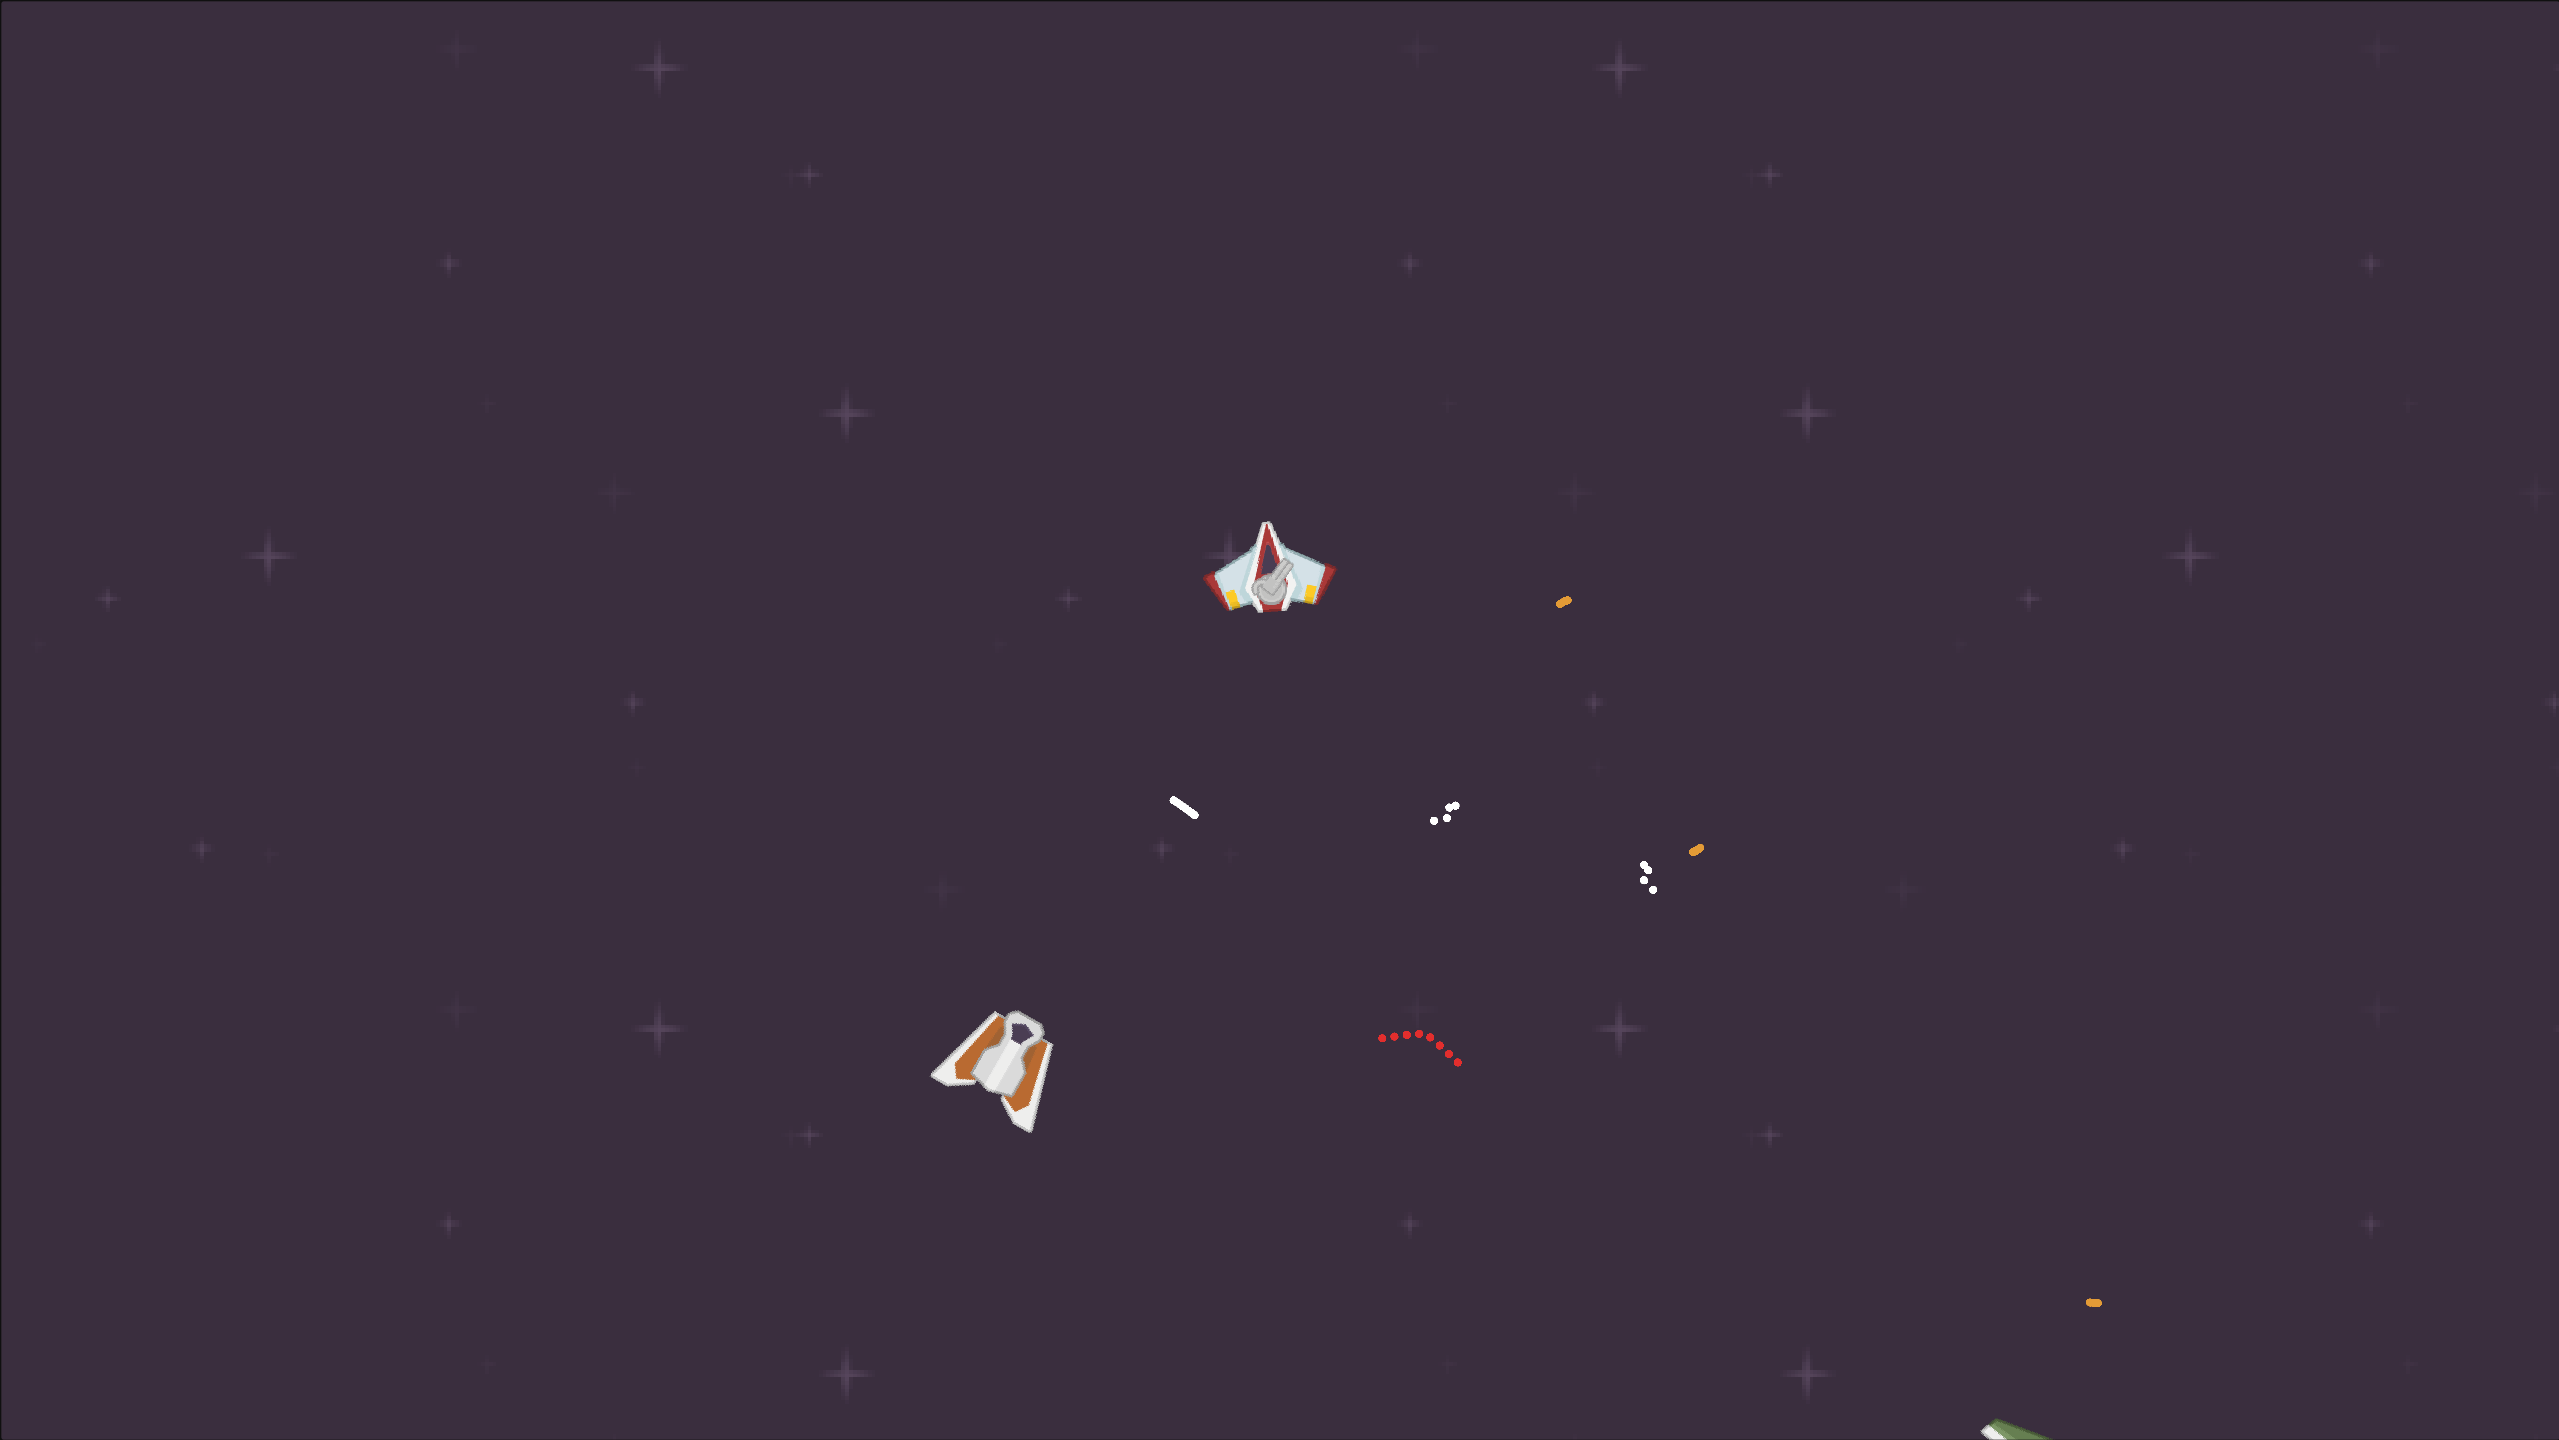
\includegraphics{images/SpaceShooter}
            }

            \caption{
                \label{SpaceShooter}
                Space Shooter.
            }
        \end {center}
    \end {figure}


\end{enumerate}

Ассеты для создания двух игр были получены с таких сайтов, как:
\begin{enumerate}
    \item Unity Asset Store\cite{s4}
    \item opengameart.org\cite{s5}
    \item itch.io\cite{s6}
\end{enumerate}

\pagebreak


\subsection{Unity Asset Store}

Для публикации было написано описание ассета, добавлены видео и скриншоты. На момент написания отчета ассет проходит модерацию.

\begin{figure}[ht]
    \begin{center}
        \scalebox{0.3}{
            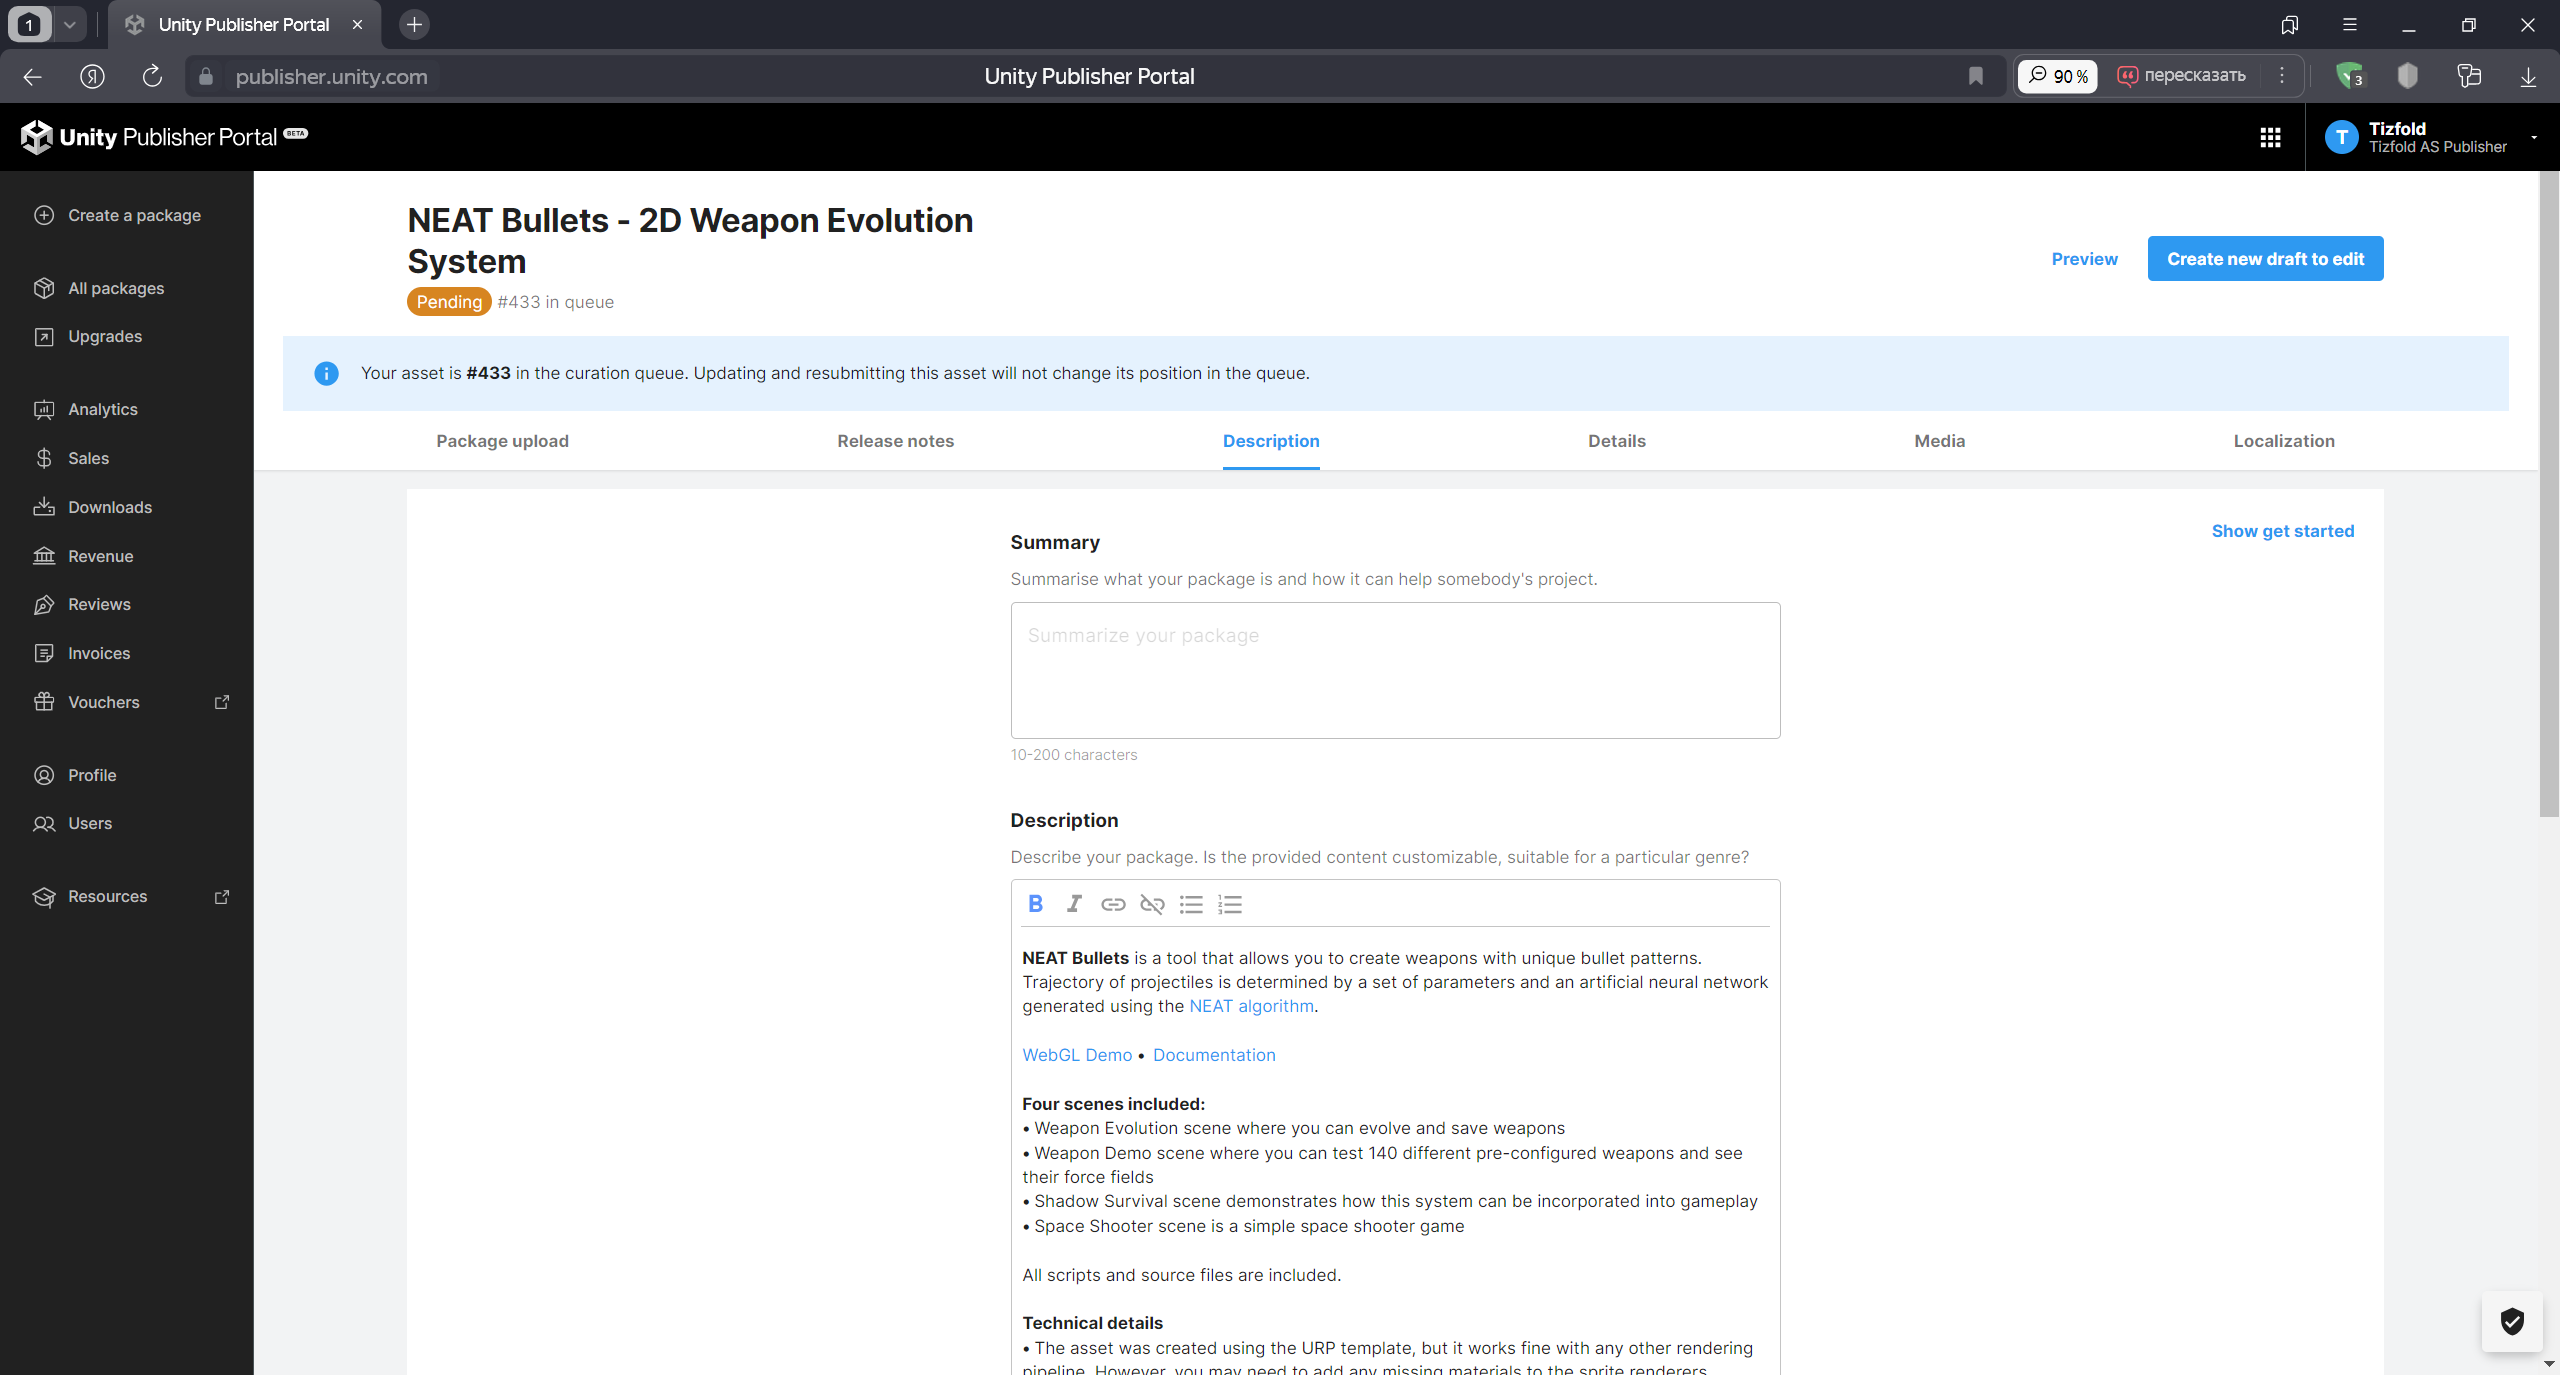
\includegraphics{images/PublisherPortal}
        }

        \caption{
            \label{PublisherPortal}
            Publisher Portal.
        }
    \end {center}
\end {figure}